% mnras_template.tex 
%
% LaTeX template for creating an MNRAS paper
%
% v3.0 released 14 May 2015
% (version numbers match those of mnras.cls)
%
% Copyright (C) Royal Astronomical Society 2015
% Authors:
% Keith T. Smith (Royal Astronomical Society)

% Change log
%
% v3.0 May 2015
%    Renamed to match the new package name
%    Version number matches mnras.cls
%    A few minor tweaks to wording
% v1.0 September 2013
%    Beta testing only - never publicly released
%    First version: a simple (ish) template for creating an MNRAS paper

%%%%%%%%%%%%%%%%%%%%%%%%%%%%%%%%%%%%%%%%%%%%%%%%%%
% Basic setup. Most papers should leave these options alone.
\documentclass[fleqn,usenatbib]{mnras}

% MNRAS is set in Times font. If you don't have this installed (most LaTeX
% installations will be fine) or prefer the old Computer Modern fonts, comment
% out the following line
\usepackage{newtxtext,newtxmath}
% Depending on your LaTeX fonts installation, you might get better results with one of these:
%\usepackage{mathptmx}
%\usepackage{txfonts}

% Use vector fonts, so it zooms properly in on-screen viewing software
% Don't change these lines unless you know what you are doing
\usepackage[T1]{fontenc}
\usepackage{ae,aecompl}


%%%%% AUTHORS - PLACE YOUR OWN PACKAGES HERE %%%%%

% Only include extra packages if you really need them. Common packages are:
\usepackage{graphicx}	% Including figure files
\usepackage{amsmath}	% Advanced maths commands
\usepackage{amssymb}	% Extra maths symbols

%%%%%%%%%%%%%%%%%%%%%%%%%%%%%%%%%%%%%%%%%%%%%%%%%%

%%%%% AUTHORS - PLACE YOUR OWN COMMANDS HERE %%%%%

% Please keep new commands to a minimum, and use \newcommand not \def to avoid
% overwriting existing commands. Example:
%\newcommand{\pcm}{\,cm$^{-2}$}	% per cm-squared

%%%%%%%%%%%%%%%%%%%%%%%%%%%%%%%%%%%%%%%%%%%%%%%%%%

%%%%%%%%%%%%%%%%%%% TITLE PAGE %%%%%%%%%%%%%%%%%%%

% Title of the paper, and the short title which is used in the headers.
% Keep the title short and informative.
\title[Hercules-Aquila and Virgo Clouds with Gaia DR2]{Hercules-Aquila
  and Virgo Clouds with Gaia DR2. Evidence for a common origin}

% The list of authors, and the short list which is used in the headers.
% If you need two or more lines of authors, add an extra line using \newauthor
\author[K. T. Smith et al.]{
Keith T. Smith,$^{1}$\thanks{E-mail: mn@ras.org.uk (KTS)}
A. N. Other,$^{2}$
Third Author$^{2,3}$
and Fourth Author$^{3}$
\\
% List of institutions
$^{1}$Royal Astronomical Society, Burlington House, Piccadilly, London W1J 0BQ, UK\\
$^{2}$Department, Institution, Street Address, City Postal Code, Country\\
$^{3}$Another Department, Different Institution, Street Address, City Postal Code, Country
}

% These dates will be filled out by the publisher
\date{Accepted XXX. Received YYY; in original form ZZZ}

% Enter the current year, for the copyright statements etc.
\pubyear{2018}

% Don't change these lines
\begin{document}
\label{firstpage}
\pagerange{\pageref{firstpage}--\pageref{lastpage}}
\maketitle

% Abstract of the paper
\begin{abstract}
200 words for Letters.
No references should appear in the abstract.
\end{abstract}

% Select between one and six entries from the list of approved keywords.
% Don't make up new ones.
\begin{keywords}
keyword1 -- keyword2 -- keyword3
\end{keywords}

%%%%%%%%%%%%%%%%%%%%%%%%%%%%%%%%%%%%%%%%%%%%%%%%%%

%%%%%%%%%%%%%%%%% BODY OF PAPER %%%%%%%%%%%%%%%%%%

\section{Introduction}

How do you hide the evidence for a massive impact event that caused
the extinction of most of the dinosaurs as well as 75\% of all species
on Earth? You bury it deep under the sea, covered with a layer of
sediment taller than the Empire State Building
\citep[][]{Hildebrand1991}. Without the discovery of the giant
Chicxulub crater, the meteorite impact hypothesis would remain a neat
theory supported by striking but indirect evidence. A hypothesis of an
ancient dramatic collision between the Milky Way and an unidentified
massive dwarf galaxy was put forward by \citet{Deason2013} to explain
a particular feature in the overall stellar halo density profile
\citep[][]{Wa09,De11}. Most recently, through a study of a portion of
the nearby stellar halo, \citet{Belokurov2018} demonstrated that the
great impactor must have collided with the young Milky Way on a nearly
radial orbit, thus swamping the inner stellar halo with metal-rich
material with orbital anisotropy \citep[see][]{Binney2008} close to
unity. Merger events like this tend to leave behind a battery of
debris clouds and shells \citep[see][]{Amorisco2015,Hendel2015}, which
- akin to the peak rings of impact craters \citep[see
  e.g.][]{Morgan2016} - if discovered could help to reconstruct the
collision as well as pin down the properties of the progenitor
\citep[e.g][]{Sanderson2013,Johnston2016}.

Before the Data Release 2 \citep[][]{Brown2018} of the ESA's Gaia
mission \citep[][]{Prusti2016}, five large and diffuse cloud-like
structures had been discovered in the Galaxy's halo. These include:
the Virgo Over-Density
\citep[VOD,][]{Vivas2001,Newberg2002,Duffau2006,Juric2008,Bonaca2012},
the Hercules-Aquila Cloud \citep[HAC,][]{Be07,Simion2014}, the
Trinagulum-Andromeda structure
\citep[Tri-And,][]{Rocha2004,Majewski2004,Deason2014}, the Pisces
Over-density \citep[][]{Sesar2007,Wa09,Nie2015} and the
Eridanus-Phoenix over-density \citep[Eri-Pho,][]{Li2016}. According to
the most recent investigations, Tri-And likely comprises of Galactic
disc stars kicked out of the plane in a recent interaction with a
dwarf galaxy, probably the Sagittarius dSph
\citep[e.g.][]{Pr15,Bergemann2018,Hayes2018}. Of the remaining four,
the Pisces overdensity clearly stands out as it reaches much larger
Galacto-centric distances. On the other hand, the VOD, HAC and Eri-Pho
structures occupy a very similar range of distances, between 10 and 20
kpc from the Galactic center. This lead \citet{Li2016} to suggest that
these three Clouds could all be part of one merger event, a galaxy
accreted onto the Milky Way on a polar orbit \citep[see
  also][]{Juric2008}.

As demonstrated by the recent re-interpretation of the Monoceros Ring
(and the associated sub-structures) and the Tri-And, deciphering the
nature of halo over-densities is often impossible without either
high-resolution spectroscopy \citep[e.g.][]{Bergemann2018} or accurate
astrometry \citep[e.g.][]{deBoer2018,Deason2018}. In this Letter, we
look for clues to the formation of the Hercules-Aquila and Virgo
Clouds using proper motions provided as part of the Gaia DR2. At our
disposal are highly pure samples of members of each Cloud, namely the
RR Lyrae stars that i) are co-spatial with HAC and VOD in 3-D and ii)
that have their line-of-sight velocities measured. By complementing
the publicly available 4-D data with the GDR2 proper motions, we build
a large tracer set with complete 6-D phase space information and study
the make-up of each structure using the orbital properties of the
constituent stars.

\section{Data and analysis}
%
\begin{figure*}
	% To include a figure from a file named example.*
	% Allowable file formats are eps or ps if compiling using latex
	% or pdf, png, jpg if compiling using pdflatex
	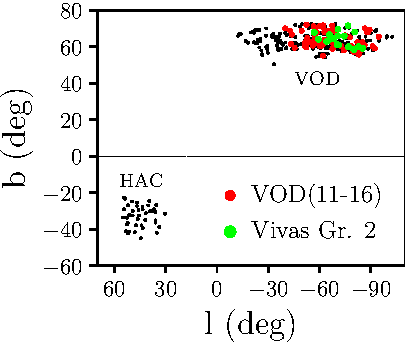
\includegraphics[scale=0.61]{lb.pdf}
	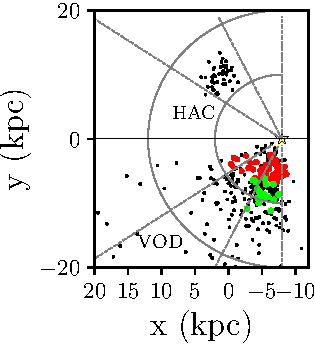
\includegraphics[scale=0.61]{xy.pdf}
	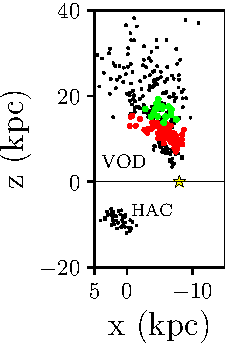
\includegraphics[scale=0.61]{xz.pdf}
    \caption{Spatial distribution of the RR Lyrae used in this work with full 6-D phase space measurements, in Galactic coordinates (left panel) and in the $x-y$ (middle) and $y-z$ (right) planes.  The HAC field contains 44 RR Lyrae which likely belong to the Cloud with measured line-of-sight  velocities (Simion et al. 2018) and  Gaia DR2 proper motions. The VOD field contains 411 RRL which belong to several halo associations, including the Sagittarius stream and the VOD, with line-of-sight velocities provided by Vivas et al. 2016 and proper motions from Gaia DR2. In particular we mark group 2, a `high significance' kinematical group, which contains 18 stars (green circles). The semi-circles are centred on the Sun's position and have radius of 10 and 20 kpc. The Sun (yellow star) is located at (x$_{\odot}$, y$_{\odot}$, z$_{\odot})= $ (0,-8,0) kpc and the Galactic centre at (0,0,0) - black circle.  }
    \label{fig:lb}
\end{figure*}
\subsection{4-D data}
The Hercules-Aquila  and Virgo Clouds are revealed unambiguously as overdensities of RR Lyrae  in the halo, which peak at similar heliocentric distances,  $\sim$17 kpc (HAC: \citealt{Simion2014}) and $\sim$19 kpc (VOD: \citealt{Vivas2006, Duffau2014, Vivas2016}) respectively, but in opposite quadrants (e.g. their distribution in Galactic coordinates in Fig. \ref{fig:lb}). Other tracers (e.g. BHBs, MSTO, K giants) have been used to pin down the morphology of  the Clouds with slightly inconsistent results between them, caused by poor distance determination, scarcity or simply trace the structures differently; therefore, the most recent kinematic follow-ups of the clouds have used RR Lyrae selected in the vicinity of the overdensities peak: 
\begin{itemize}
\item \citet{Simion2018}  provide a table of 46 RRL with radial velocity measurements (45 observed with MDM and 1 from SDSS) with heliocentric distances between 15 and 18 kpc;
\item \cite{Vivas2016} compiled a catalog of 412 RRL in the region of the sky covered by the VOD with distances between 4 and 75 kpc from the Sun with radial velocity measurements from La Silla-QUEST, QUEST, CRTS and LINEAR. 
\end{itemize}
%
\subsection{6-D data: velocity distributions}
From the two tables of RR Lyrae with 4D measurements, 44 stars in the HAC field and 411 in the VOD field have matches in GDR2 within 2'' and proper motion measurements. The only star in the VOD region without proper motion belongs to a `high-significance' kinematical group (group 1), likely the Sagittarius stream, identified by \cite{Vivas2016}. This group contains 113 stars (112 with proper motions)  which we remove from the VOD sample as a major contaminant of the field. The spatial distribution of the remaining stars (44 from \citealt{Simion2018} and 299 from \citealt{Vivas2016}) with full 6-D phase space measurements is illustrated in Figure \ref{fig:lb}, in Galactic coordinates (left panel) and in the (x-y) Galactic plane and the (x-z) plane, perpendicular to (x-y). We adopted a left-handed Galactic Cartesian coordinates with the Sun located at (x$_{\odot}$,y$_{\odot}$, z$_{\odot}$) = (-8,0,0) kpc, the x-axis positive in the direction of the Galactic center, y-axis oriented along the Galactic rotation and the z-axis directed towards the north Galactic pole.\\
While \citealt{Vivas2016} identify 6 significant kinematical groups in the VOD field (their table 5) only groups 1 (Sagittarius stream) and 2 (likely members of the VOD, with $\mathrm{<v_{GSR}>}= 135$ km/s) contain more than 10 stars. We mark group 2 with green circles in Figure \ref{fig:lb}. We also mark with red circles the location of a group of stars with galactocentric distances similar to the HAC sample, $11\mathrm{<r_{GC}}/$kpc$<16$ as we intend to follow their velocity distribution and orbital properties.\\
%
%
%
%
\begin{figure}
	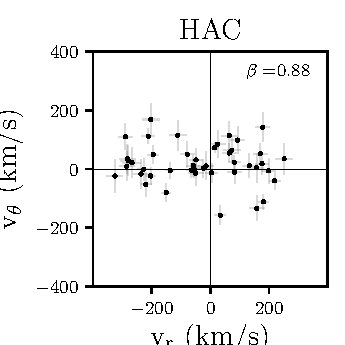
\includegraphics[scale=0.545]{HAC_velocities_vphi.pdf}
	\hspace{-0.25cm}
    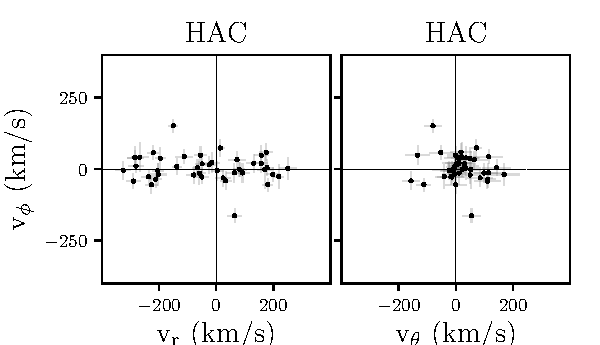
\includegraphics[scale=0.545]{HAC_velocities_vtheta.pdf} \\
  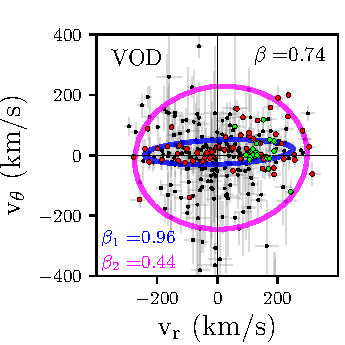
\includegraphics[scale=0.545]{VOD_velocities_vphi.pdf}
  \hspace{-0.25cm}
    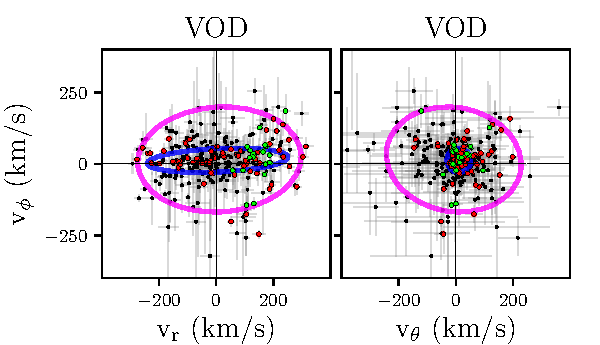
\includegraphics[scale=0.545]{VOD_velocities_vtheta.pdf}   \\
\vspace{-0.3cm}
    \caption{RRL velocity distribution in spherical polar coordinates ($v_{r}$, $v_{\theta}$, $v_{\phi}$  are the radial, azimuthal and polar components respectively) in the HAC field (top row) and the VOD field (middle and bottom rows). The error on the velocity components of each star $i $, [$\sigma^{i}_{v_{r}}$, $\sigma^{i}_{v_{\theta}}$, $\sigma^{i}_{v_{\phi}}$], has been propagated by randomly drawing 1000 stars from a multivariate Gaussian distribution with mean the measurement (ra$^{i}$, dec$^{i}$, d$^{i}$, pmra$^{i}$, pmdec$^{i}$, $v^{i}_{h}$) and full covariance matrix (takes into account the covariances between ra,dec and proper motions). The orbital anisotropy, is highly radial in the HAC field ($\beta = 0.91 \pm 0.03$) where the stars are most likely members of the Cloud and mildly radial in the VOD field ($\beta = 0.74 \pm 0.04$) in which stars span a much wider range of distances (see Fig. \ref{fig:lb}). }
    \label{fig:vel}
\end{figure}
%
\begin{figure}
	\hspace{-0.3cm}
	        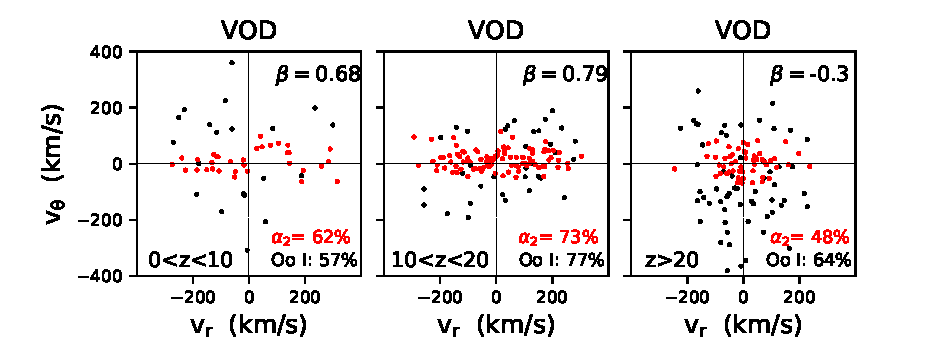
\includegraphics[scale=0.555]{VOD_velocities_vphi_zcuts.pdf}
\vspace{-0.4cm}
   \caption{Radial versus azimuthal velocity in the VOD field, in three distance ranges above the Galactic plane. The fraction of RR Lyrae of Oosterhoff type I is reported in each panel. }
    \label{fig:VOD_vel}
\end{figure}
%
The velocity distribution in the VOD and HAC fields is shown in Fig. \ref{fig:vel} in spherical polar coordinates, where $v_{r}$, $v_{\theta}$, $v_{\phi}$  are the radial, azimuthal and polar components respectively. `Group 2' stars (lime) form a group at $v_{r} = 135$ km/s as expected, while the stars at intermediate $\mathrm{r_{GC}}$ (red) seem to have a velocity distribution very similar to HAC, shown in the top panels. To estimate the error on each velocity component we resample the data 1000 times  from a multivariate Gaussian distribution with mean the measurement \{$\alpha$, $\delta$, $\mathrm{d_{helio}}$, $\mu_{\alpha} \mathrm{cos(\delta)}$, $\mu_{\delta}$, $\mathrm{v_{helio}}$\}$_{i}$ and full covariance matrix which takes into account the covariances between the right ascension $\alpha$, declination $\delta$ and proper motions, provided by GDR2. We take the standard deviation of the resulting \{$v_{r}$, $v_{\theta}$, $v_{\phi}$\} distributions as the upper limit of the velocity uncertainties and show them in Fig. \ref{fig:vel}. \\ %add comments on the size of the errorbars; standard deviation works well I think here, distributions quite gaussian. didn't work well for the anisotropy later on, there I used the percentiles 
We calculate the velocity anisotropy in the two fields, keeping in mind the two samples span very different distance ranges. 
%(\textit{need to add 1 sentence about anisotropy and formula}). 
We compute the median and standard deviation over 500 non parametric bootstrap resampling trials, where each trial was modelled with a velocity ellipsoid using the Extreme Deconvolution module implemented in  $\mathrm{astroML}$ \citep{astroML}. We find the HAC stars have radially biased orbits ($\beta = 0.91 \pm 0.03$) while the VOD stars have slightly less radial orbits ($\beta = 0.74 \pm 0.04$).\\
We fit a model with two multivariate Gaussians to the VOD velocity ellipsoid using Extreme Deconvolution and obtain  $\beta_{1}= 0.96^{+0.02}_{-0.44}$ (marked in magenta in Fig. \ref{fig:vel}) and $\beta_{2}=0.44^{+0.45}_{-0.20}$ (blue).

Fig. \ref{fig:VOD_vel} shows the behaviour of the VOD azimuthal $v_{\theta}$ and radial $v_{r}$ velocity distributions in 3 distanges ranges above the Galactic plane. In each slice we have calculated the fraction of Oosterhoff type I (Oo I) RR Lyrae, using equations 1 and 2 in \citet{Be2018} to classify the RRL into two types. According to this classification, Oosterhoff type II (Oo II) RR Lyrae will incude both Oo II and Intermediate objects. In the 10$<$z/kpc$<$20 range, where the velocity anisotropy is the highest ($\beta = 0.84 \pm 0.03$) approaching the value in the HAC field, the Oo I type dominates  (77\%). In the same slice, 73\% of the stars belong to the more squashed (or `sausage' looking) velocity ellipsoid. The same behaviour but less accentuated can be noticed in the 0$<$z/kpc$<$10 slice where the anisotropy $\beta = 0.7 \pm 0.1$ is lower but the fraction of Oo I stars decreases drammatically to 57\%. Further from the plane, at  z$>$20 kpc, the velocity ellipsoid is almost isotropic with $\beta = -0.1 \pm 0.2$. Here, the $\beta$ value may still be affected by the presence of the Sagittarius stream in the field. Group 2 and red points are all located at $z<20$ kpc, with the red points following an anisotropic velocity distribution.
 % 
\subsection{Orbital properties of the HAC and VOD}
%
\begin{figure}
	% To include a figure from a file named example.*
	% Allowable file formats are eps or ps if compiling using latex
	% or pdf, png, jpg if compiling using pdflatex
	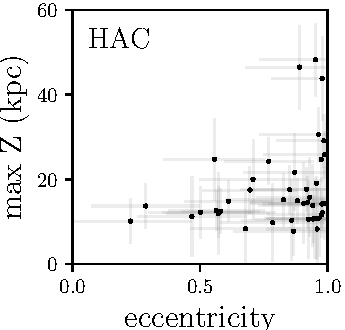
\includegraphics[scale=0.472]{HAC_orbits_ecc_z.pdf}
    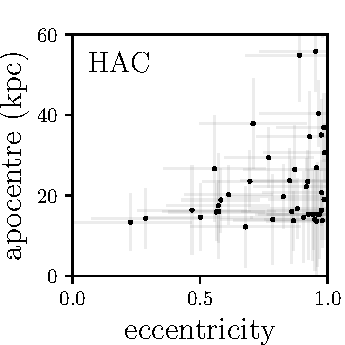
\includegraphics[scale=0.472]{HAC_orbits_apo_ecc.pdf} 
  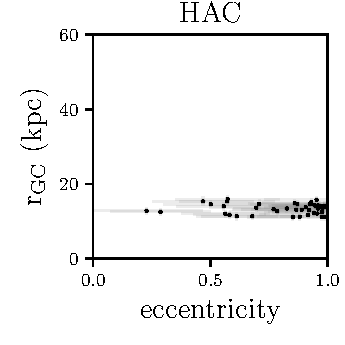
\includegraphics[scale=0.472]{HAC_orbits_ecc_r.pdf} \\
	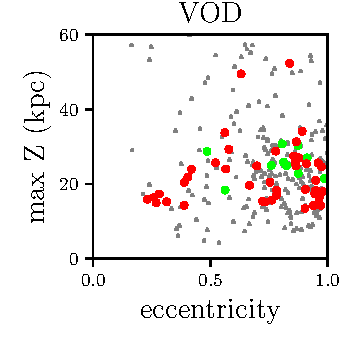
\includegraphics[scale=0.472]{VOD_orbits_ecc_z.pdf}
    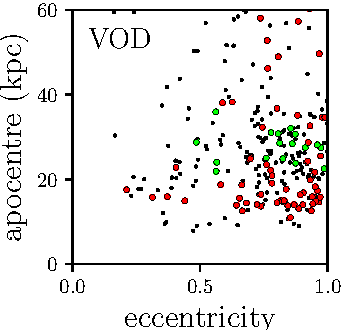
\includegraphics[scale=0.472]{VOD_orbits_apo_ecc.pdf} 
  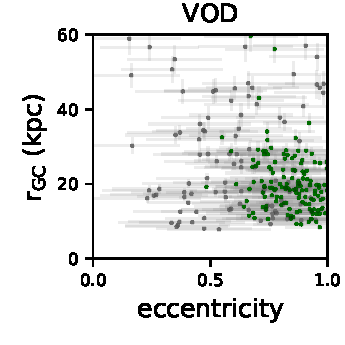
\includegraphics[scale=0.472]{VOD_orbits_ecc_r.pdf} \\
              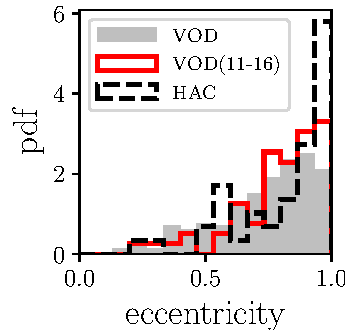
\includegraphics[scale=0.472]{eccentricities.pdf} 
    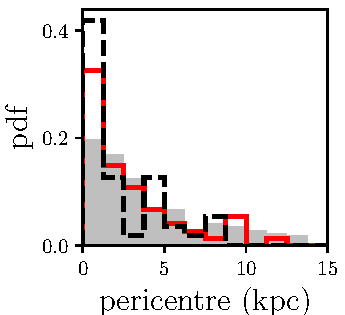
\includegraphics[scale=0.472]{pericentres.pdf} 
                          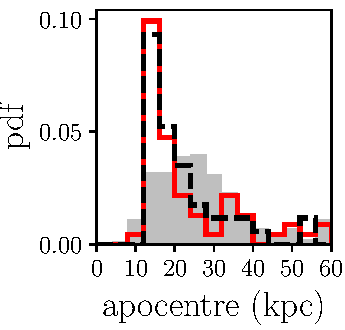
\includegraphics[scale=0.472]{apocentres.pdf} 
  \caption{ Orbital properties of the stars in the HAC and VOD fields. `group 2' has similar orbital properties to the HAC, however it does not display a sausage velocity distribution (see middle row figure 2) - they are concentrated at $vr =  135 $km/s as calculated by Vivas et al. 2016. }
    \label{fig:orbits}
    
    \end{figure}
   %
For orbit integration we use the $\mathrm{galpy}$ package \citet{Bovy2015} in the recommended  $\mathrm{MWPotential2014}$ model for the Galactic potential which is composed of a Miyamoto-Nagai disc, a bulge with a power-law density profile that is exponentially cut-off, and a dark matter halo described by a NFW potential. The parameters are given in \citet{Bovy2015}, table 1. The resulting orbital parameters of the HAC and VOD are given in Fig \ref{fig:orbits}. To compute the errors (not shown for VOD to simply the figure) we integrated 500 orbits for each star where the orbits were initialised on parameters resampled from data, as in the previous section. The pdfs of the eccentricities, apocentres and pericentres are also shown.
If the HAC orbits are clearly highly eccentric, we find that the majority of stars in VOD are also on quite eccentric orbits: in particular, the stars with $11<\mathrm{r_{GC}}$/kpc$<16$ (in red), follow closely the HAC orbital properties.
%
\section{Are the VOD and the HAC related?}
In this section we discuss the possible connection between the two clouds. 
We use the 6-D phase space measurements as initial conditions for backward orbit integration. We integrate the orbits for 8 Gyrs %here need to discuss why.
and show them in Fig. \ref{fig:backorbits}.


\begin{figure*}
	     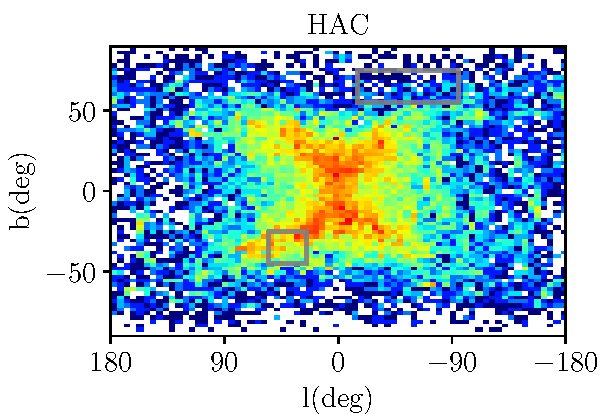
\includegraphics[scale=0.52]{HAC_orbits_8Gyrs_lb_defaultmass.pdf}
	     	     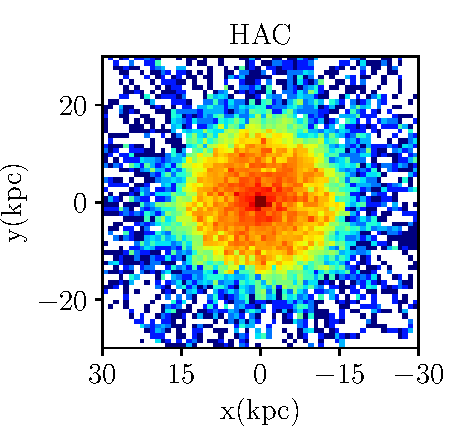
\includegraphics[scale=0.52]{HAC_orbits_8Gyrs_xy_defaultmass.pdf}
	     	     	     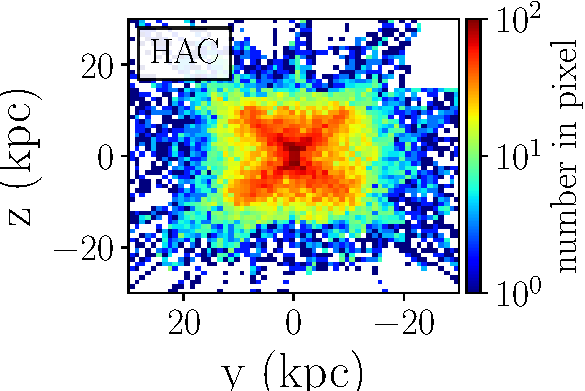
\includegraphics[scale=0.52]{HAC_orbits_8Gyrs_yz_defaultmass.pdf}
	     	     	     	     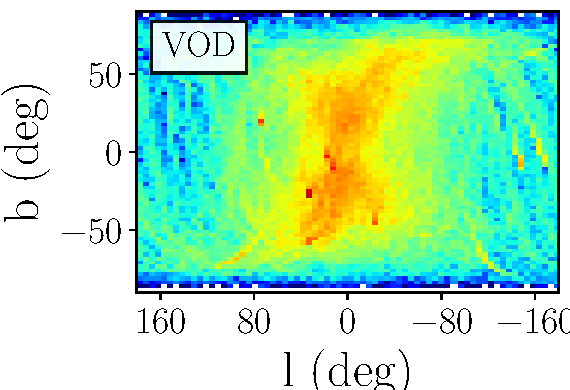
\includegraphics[scale=0.52]{VOD_orbits_8Gyrs_lb_defaultmass.pdf}
	     	     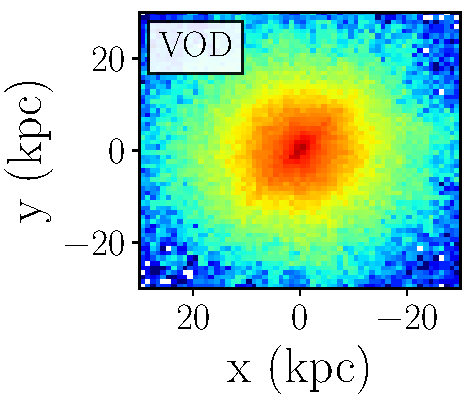
\includegraphics[scale=0.52]{VOD_orbits_8Gyrs_xy_defaultmass.pdf}
	     	     	     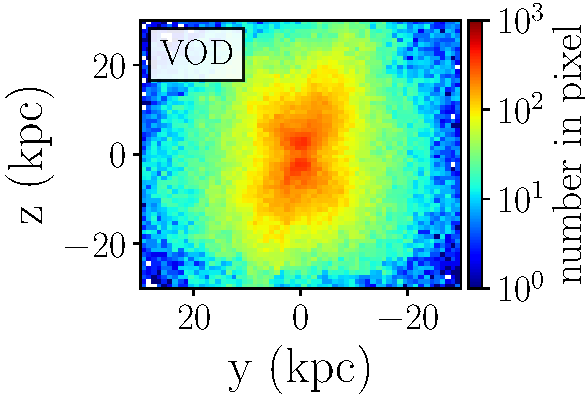
\includegraphics[scale=0.52]{VOD_orbits_8Gyrs_yz_defaultmass.pdf}
	     	     	     	     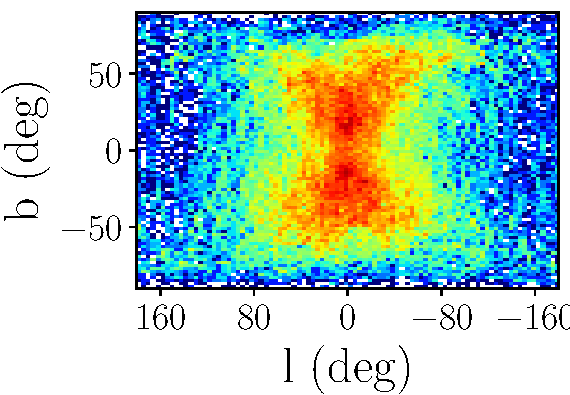
\includegraphics[scale=0.52]{VOD_orbits_8Gyrs_lb_sausage.pdf}
	     	     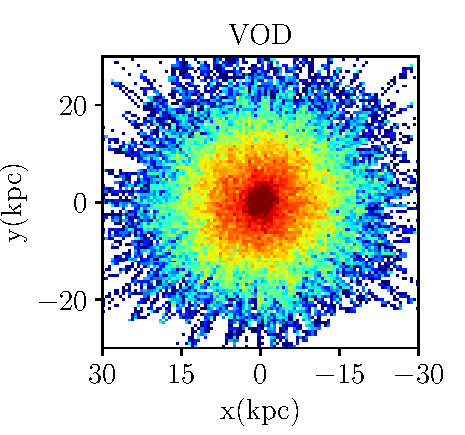
\includegraphics[scale=0.52]{VOD_orbits_8Gyrs_xy_sausage.pdf}
	     	     	     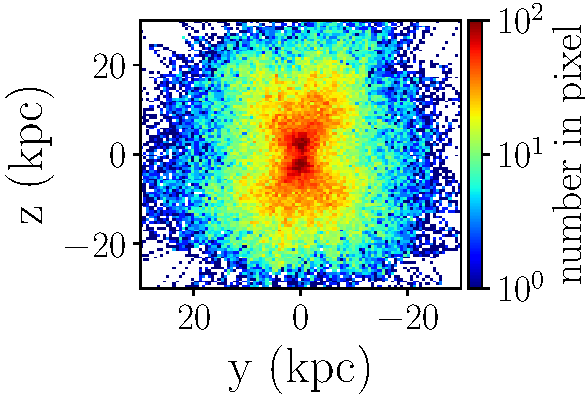
\includegraphics[scale=0.52]{VOD_orbits_8Gyrs_yz_sausage.pdf}
   \caption{The backward orbit integration for HAC (top panels) and VOD (bottom panels) for 8 Gyrs look back time. We use $M_{vir} = 0.8 \times 10^{12} M_{\odot}$, the default galpy value . log(N) shown, notice the change in colour scale between top and bottom rows. The present day loci of  HAC and VOD are marked with gray rectangles. The initial conditions of 44 stars with heliocentric distances between 15 and 18 kpc were used for the HAC backward orbit integration and of 299 stars with heliocentric distances between 4 and 75 kpc for the VOD orbit integration.}
    \label{fig:backorbits}
\end{figure*}
\begin{figure}
	% To include a figure from a file named example.*
	% Allowable file formats are eps or ps if compiling using latex
	% or pdf, png, jpg if compiling using pdflatex
	       	       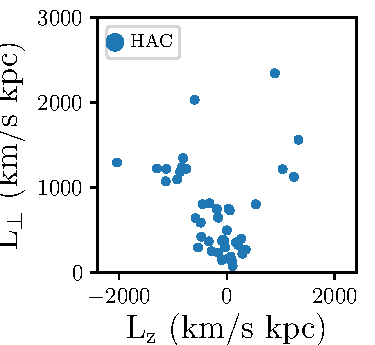
\includegraphics[scale=0.52]{HAC_Lz_Lp.pdf}
	       	       	       	       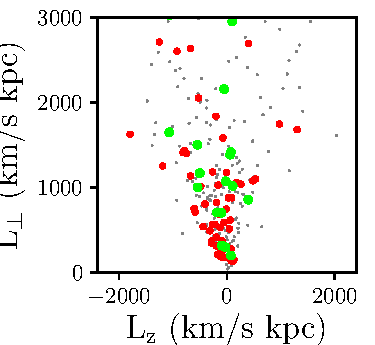
\includegraphics[scale=0.52]{VOD_Lz_Lp.pdf}
   \caption{EXTRA: angular momentum - I can combine these two and also add another panel with energy vs total L when I figure out the energy.}
    \label{fig:l}
\end{figure}
\section{Conclusions}

Using a sample of $\sim$500 RR Lyrae with full 6-D phase space
information, we have studied the orbital properties of the
Hercules-Aquila and Virgo Clouds. Both Clouds appear dominated by
stars on highly eccentric orbits. Assuming that the kinematics of each
structure is well described by a single Gaussian, the orbital
anisotropy of the HAC is $\beta=0.91$ and for the VOD,
$\beta=0.74$. Note, however that the original criteria applied to the
RR Lyrae stars to select targets for spectroscopic follow-up differ
drastically between the HAC and the VOD datasets. The HAC sample
covers a very limited region in the of $l,b, D$ space, while the VOD
dataset spans a wide range of longitudes, latitudes and heliocentric
distances. It is therefore likely that the VOD dataset contains a
mixture of several halo sub-structures \citep[see][for a detailed
  discussion]{Vivas2016}. For the entirety of the analysis described
here, we made sure to cull the probable Sgr stream
members. Additionally, we explore how the VOD's make-up changes with
Galactic height and demonstrate that for $|z|<20$ kpc, the VOD orbital
anisotropy is $\beta\sim 0.84$, while above this threshold, it quickly
changes to $\beta\sim0$. We conclude therefore, that an assumption of
a single Gaussian for the entire VOD sample is not
appropriate. Modeling the kinematics of the VOD stars with a mixture
of 2 multi-variate Gaussians, we show that two thirds of the VOD
sample are the stars with $\beta=0.96$, while the remainder has
$\beta=0.44$, in good agreement with the local measurement presented
in \citet{Belokurov2018}.

As revealed by Gaia, the two structures are composed of stars on
nearly radial orbits, with peaks in the eccentricity distribution at
0.9 (0.8) for the HAC (VOD). The distributions of the peri-centric and
apo-centric distances also match: the stars in the Clouds turn around
at $1-3$ and $15-30$ kpc. Not only the HAC and the VOD look alike
kinematically, their orbital composition is in perfect agreement with
the stellar halo properties as analysed locally by
\citet{Belokurov2018} and globally (out to 40 kpc) by
\citet{Deason2018pileup}. As these authors demonstrate, the inner halo
is dominated by metal-rich debris from an old and massive accretion
event. In particular, \citet{Belokurov2018} use Cosmological
simulations of Milky Way halo formation, to bracket the time of the
merger - between 8 and 11 Gyr ago - and its mass, which they show to
be in excess of $10^{10} M_{\odot}$. The tell-tale sign of this
dramatic head-on collision is the particular shape of the
corresponding stellar velocity ellipsoid, which is stretched so much
in the radial direction compared to the tangential ones, that it
resembles a sausage. An alternative view of this merger can be found
in \citet{actionhalo}, where the local stellar halo is mapped out in
the action space. Here, the metal-rich stars are shown have extended
radial action distribution in addition to a prominent spray of
material on retrograde orbits. The high mass of the progenitor is
evidenced not only by the metallicity distribution of its likely
member or the numerical simulations of halo formation, but also by a
sizeable number of Globular Clusters that could be attributed to the
same event \citep[see][]{sausagegc}.


\section*{Acknowledgements}

The Acknowledgements section is not numbered. Here you can thank helpful
colleagues, acknowledge funding agencies, telescopes and facilities used etc.
Try to keep it short.

%%%%%%%%%%%%%%%%%%%%%%%%%%%%%%%%%%%%%%%%%%%%%%%%%%

%%%%%%%%%%%%%%%%%%%% REFERENCES %%%%%%%%%%%%%%%%%%

% The best way to enter references is to use BibTeX:
%citations used: 
\bibliographystyle{mn2e}
\bibliography{bibl}  %the same name as the tex file
%%%%%%%%%%%%%%%%%%%%%%%%%%%%%%%%%%%%%%%%%%%%%%%%%%
% Don't change these lines
\bsp	% typesetting comment
\label{lastpage}
\end{document}
% End of mnras_template.tex
